\documentclass[conference]{IEEEtran}
\IEEEoverridecommandlockouts
% The preceding line is only needed to identify author in the first page
% if using IEEEtran format for a conference paper; otherwise, it may be
% removed.

\usepackage{cite}
\usepackage{amsmath,amssymb,amsfonts}
\usepackage{algorithmic}
\usepackage{graphicx}
\usepackage{textcomp}
\usepackage{xcolor}
\usepackage{tikz}
\usepackage{pgfplots}
\usetikzlibrary{shapes,arrows,positioning,calc,decorations.pathmorphing}
\usepackage{listings}
\usepackage{xcolor}
\def\BibTeX{{\rm B\kern-.05em{\sc i\kern-.025em b}\kern-.08em
    T\kern-.1667em\lower.7ex\hbox{E}\kern-.125emX}}

\begin{document}

\title{Twinkies: A Modern Multi-Target Compiler with Static Type Checking and Foreign Function Interface Support}

\author{\IEEEauthorblockN{1\textsuperscript{st} Anonymous Author}
\IEEEauthorblockA{\textit{Department of Computer Science} \\
\textit{University}\\
City, Country \\
email@example.com}
}

\maketitle

\begin{abstract}
This paper presents Twinkies, a compiler for a statically-typed programming language that generates both C and assembly code. The compiler implements a traditional multi-phase architecture: lexical analysis, parsing, semantic analysis, IR generation, and code generation. The compiler provides static type checking with scope-based symbol resolution, automatic array bounds checking, a foreign function interface for dynamic library integration, a module system with header files, and inline assembly support. The Strategy design pattern is used in code generation to support multiple target languages. The evaluation covers correctness testing and performance analysis using test suites that exercise basic language constructs, advanced features, and FFI integration. The results show that separating concerns across compiler phases leads to maintainable code generation strategies and effective error detection.
\end{abstract}

\begin{IEEEkeywords}
compiler design, static type checking, intermediate representation, code generation, foreign function interface, transpiler
\end{IEEEkeywords}

\section{Introduction}

Finding the right balance between expressiveness, type safety, and performance remains a challenge in modern software development. High-level languages boost productivity, but sometimes you need the control that low-level languages offer. Transpilers help bridge this gap by translating source code to established targets like C, which provides both portability and performance.

Twinkies is a compiler for a statically-typed language that generates C and assembly code. The language uses C-like syntax with static typing, so it should feel familiar to developers working with imperative languages while catching errors at compile time.

The compiler uses a traditional multi-phase design. Each phase—lexical analysis, parsing, semantic analysis, IR generation, and code generation—runs independently but shares context through well-defined data structures. This separation made it easier to extend the compiler later. In code generation, the Strategy design pattern was applied, which allows switching between C and assembly output without major changes.

The main contributions include: a complete compiler implementation showing modern compiler techniques, static type checking with detailed error reporting, automatic array bounds checking with compile-time optimizations, an FFI system that works across Windows, Linux, and macOS, a module system for code organization, and a strategy-based code generation framework that supports multiple targets.

The paper is organized as follows. Section II covers related work. Section III describes the system architecture. Section IV explains how each phase was implemented. Section V presents the evaluation results. Section VI discusses trade-offs and limitations. Section VII concludes and suggests future work.

\section{Background and Related Work}

Compiler construction has been central to computer science since the first high-level languages appeared. Most modern compilers use a multi-phase architecture, as outlined in the "Dragon Book"\cite{aho2006compilers}. The typical phases are lexical analysis, syntax analysis, semantic analysis, optimization, and code generation.

\subsection{Lexical and Syntax Analysis}

Lexical analysis converts source code into a token stream. Tokens include keywords, identifiers, literals, and operators. The Twinkies lexer was written by hand, processing characters sequentially and recognizing tokens through state transitions. This took more work than using a generator like Lex\cite{lesk1975lex}, but provides better control over error messages and token recognition.

The parser builds an abstract syntax tree from the token stream. Recursive descent parsing was chosen because it fits languages with clear precedence hierarchies\cite{grune2012parsing}. Recursive descent parsers are straightforward to write and maintain, which makes them good for research compilers.

\subsection{Semantic Analysis and Type Checking}

Semantic analysis checks language rules beyond syntax. Type checking makes sure operations use compatible types, which prevents many runtime errors. A scope-based symbol table was built using hash tables, which provides fast lookups and proper scoping\cite{cooper2011engineering}.

Research shows that static type checking cuts runtime errors significantly\cite{meyer1997object}. The type system includes primitives (int, float, double, bool, string), arrays, and function types. The compatibility rules allow safe numeric conversions but block unsafe ones.

\subsection{Intermediate Representation}

IRs separate frontend analysis from backend code generation, so one IR can target multiple languages\cite{cooper2011engineering}. Three-address code is used: each instruction has at most two operands and one result. This format makes code generation simpler and leaves room for optimization passes later.

\subsection{Code Generation}

Code generation converts IR into target code. The Strategy design pattern\cite{gamma1994design} is used to pick code generation strategies at runtime. This worked well for supporting both C and assembly output in Twinkies.

\subsection{Foreign Function Interfaces}

FFIs let programs call functions from other languages or libraries. The FFI system loads dynamic libraries on Windows, Linux, and macOS, with platform-specific code for each. Established FFI patterns were followed\cite{levy2017ownership}.

\section{System Design}

Figure~\ref{fig:architecture} shows the Twinkies compiler's multi-phase architecture. Each phase transforms the program representation, turning source code into executable target code.

\begin{figure}[!t]
\centering
\scalebox{0.7}{
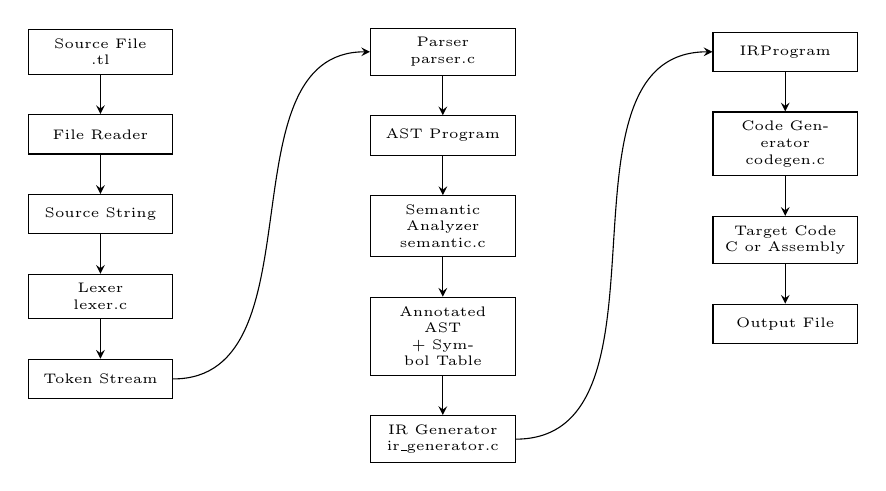
\begin{tikzpicture}[
    node distance=0.5cm,
    file/.style={rectangle, draw=black, text width=1.6cm, text centered, minimum height=0.5cm, font=\tiny},
    phase/.style={rectangle, draw=black, text width=1.6cm, text centered, minimum height=0.5cm, font=\tiny},
    data/.style={rectangle, draw=black, text width=1.6cm, text centered, minimum height=0.5cm, font=\tiny},
    arrow/.style={->, >=stealth}
]
    \node[file] (source) {Source File\\ .tl};
    \node[phase, below=of source] (reader) {File Reader};
    \node[data, below=of reader] (sourceStr) {Source String};
    \node[phase, below=of sourceStr] (lexer) {Lexer\\ lexer.c};
    \node[data, below=of lexer] (tokens) {Token Stream};
    
    \node[phase, right=of source, xshift=2cm] (parser) {Parser\\ parser.c};
    \node[data, below=of parser] (ast) {AST Program};
    \node[phase, below=of ast] (semantic) {Semantic\\ Analyzer\\ semantic.c};
    \node[data, below=of semantic] (annotated) {Annotated AST\\ + Symbol Table};
    \node[phase, below=of annotated] (irgen) {IR Generator\\ ir\_generator.c};
    
    \node[data, right=of parser, xshift=2cm] (irprog) {IRProgram};
    \node[phase, below=of irprog] (codegen) {Code Generator\\ codegen.c};
    \node[data, below=of codegen] (target) {Target Code\\ C or Assembly};
    \node[file, below=of target] (output) {Output File};
    
    \draw[arrow] (source) -- (reader);
    \draw[arrow] (reader) -- (sourceStr);
    \draw[arrow] (sourceStr) -- (lexer);
    \draw[arrow] (lexer) -- (tokens);
    \draw[arrow] (tokens) to[out=0, in=180] (parser);
    \draw[arrow] (parser) -- (ast);
    \draw[arrow] (ast) -- (semantic);
    \draw[arrow] (semantic) -- (annotated);
    \draw[arrow] (annotated) -- (irgen);
    \draw[arrow] (irgen) to[out=0, in=180] (irprog);
    \draw[arrow] (irprog) -- (codegen);
    \draw[arrow] (codegen) -- (target);
    \draw[arrow] (target) -- (output);
\end{tikzpicture}
}
\caption{Compiler architecture showing the transformation pipeline from source code to target code.}
\label{fig:architecture}
\end{figure}

\subsection{Language Syntax}

Twinkies uses C-like syntax with explicit type annotations. Functions use arrow notation for return types, variables use \texttt{let}, and control flow includes \texttt{if}, \texttt{while}, \texttt{break}, and \texttt{continue}. The language supports fixed-size arrays and built-in string operations.

\subsection{Type System}

The type system supports seven primitive types: \texttt{int}, \texttt{float}, \texttt{double}, \texttt{bool}, \texttt{string}, \texttt{void}, and \texttt{null}. Arrays are parameterized by element type and size. The type checker allows implicit conversions between numeric types but requires explicit handling for other mismatches.

\subsection{Error Handling}

The error reporting system tracks errors across all phases. Each error includes line and column numbers, severity, and suggestions. Errors are collected in a context structure that stops compilation when fatal errors occur.

\subsection{Module System}

The module system organizes code using header files (\texttt{.tlh}) and source files (\texttt{.tl}). Headers declare public interfaces; sources contain implementations. The module manager tracks dependencies and compiles modules in the right order.

\subsubsection{File Structure and Extensions}

Two file types are used: \texttt{.tl} for source code and \texttt{.tlh} for headers. A typical module has a header (e.g., \texttt{math.tlh}) declaring public functions and types, and a source file (e.g., \texttt{math.tl}) with implementations. The compiler matches headers and sources by name.

\subsubsection{Include Directive Syntax}

Modules are included with \texttt{\#include}. Two forms are supported: \texttt{\#include "local.tlh"} for local includes (searched in user-specified paths) and \texttt{\#include <system.tlh>} for system includes (searched in system paths). The compiler keeps separate search paths for local and system includes, defaulting to the current directory and common system directories.

\subsubsection{Module Compilation Process}

Compilation happens in several stages:
\begin{enumerate}
    \item \textbf{Header Parsing}: Header files are parsed first to extract public symbols. This builds a symbol table for each module with exported functions, types, and constants.
    \item \textbf{Dependency Resolution}: The module manager builds a dependency graph from \texttt{\#include} directives. It detects circular dependencies and compiles modules in topological order.
    \item \textbf{Source Compilation}: Source files compile after their dependencies, producing object files or IR. The compiler tracks compiled modules to avoid duplicate work.
    \item \textbf{Linking}: All compiled modules link together, with the main module as the entry point.
\end{enumerate}

\subsubsection{Dependency Resolution}

The module manager keeps a dependency graph where each module tracks its direct dependencies. When compiling a module, all dependencies compile first. File modification timestamps are used to decide if recompilation is needed: if a header or dependency is newer than the compiled output, the module is recompiled. This incremental approach speeds up builds for large projects.

\section{Implementation}

This section explains how each compiler phase was implemented and the key design decisions.

\subsection{Compiler Architecture and Code Organization}

The code is organized into several directories:
\begin{itemize}
    \item \textbf{\texttt{src/frontend/}}: Lexical analysis, parsing, and AST construction. Contains \texttt{lexer/}, \texttt{parser/}, and \texttt{ast/} subdirectories.
    \item \textbf{\texttt{src/analysis/}}: Semantic analysis and type checking in \texttt{semantic/}.
    \item \textbf{\texttt{src/backend/}}: IR generation and code generation. Has \texttt{ir/} for intermediate representation and \texttt{codegen/} for code generation strategies.
    \item \textbf{\texttt{src/modules/}}: Module system and FFI support, with subdirectories for module management and FFI configuration.
    \item \textbf{\texttt{src/common/}}: Shared utilities, error handling, memory management, and command-line flags.
\end{itemize}

Header files in \texttt{include/} define clean interfaces for each module, which helps with separation of concerns and makes testing easier.

\subsection{Build System}

A Makefile-based build system is used with three configurations:
\begin{itemize}
    \item \textbf{Debug Build}: Uses \texttt{-g -O0 -DDEBUG} for development and debugging.
    \item \textbf{Release Build}: Uses \texttt{-O2 -DNDEBUG} for optimized production code.
    \item \textbf{Standard Build}: Default build with \texttt{-Wall -Wextra -std=c99} for warnings and C99 compliance.
\end{itemize}

The build system finds source files using wildcards, compiles them to object files in \texttt{build/}, and links them into the final executable. Dependencies are tracked to rebuild in the correct order when files change.

\subsection{Command-Line Interface}

The compiler supports these command-line options:
\begin{itemize}
    \item \textbf{\texttt{-o <file>}}: Output file name.
    \item \textbf{\texttt{--asm}}: Generate assembly instead of C.
    \item \textbf{\texttt{--modules}}: Enable module system compilation.
    \item \textbf{\texttt{--debug}}: Show debug output with phase details.
    \item \textbf{\texttt{--verbose}}: Verbose compilation output.
    \item \textbf{\texttt{--tokens}}: Print token stream after lexical analysis.
    \item \textbf{\texttt{--ast}}: Print abstract syntax tree after parsing.
    \item \textbf{\texttt{--ir}}: Print intermediate representation after IR generation.
    \item \textbf{\texttt{--dump-ast-json}}: Export AST as JSON for tooling.
    \item \textbf{\texttt{--memory}}: Show memory allocation statistics.
    \item \textbf{\texttt{-I <path>}}: Add directory to module include path.
    \item \textbf{\texttt{--modules -o <dir>}}: Output directory for module compilation.
\end{itemize}

You can compile multiple input files into one output. The compiler combines their ASTs before semantic analysis, so multi-file projects work without a separate linking step.

\subsection{Development Tools}

\subsubsection{VS Code Extension}

A VS Code syntax highlighting extension was built for Twinkies. It recognizes \texttt{.tl} and \texttt{.tlh} files and highlights keywords, operators, literals, and comments. The extension ships as a \texttt{.vsix} package for direct installation.

\subsubsection{Debugging and Profiling}

The compiler includes debugging and profiling tools:
\begin{itemize}
    \item \textbf{Memory Profiling}: The \texttt{--memory} flag tracks all allocations and deallocations, showing total memory used, allocation count, and potential leaks. This was useful for identifying memory issues during development.
    \item \textbf{Debug Mode}: The \texttt{--debug} flag enables detailed logging showing phase transitions, intermediate results, and internal state.
    \item \textbf{Verbose Output}: The \texttt{--verbose} flag shows compilation progress, including files being processed, modules being loaded, and timing.
\end{itemize}

\subsection{Error Recovery Mechanisms}

Several error recovery strategies were implemented to provide useful diagnostics:
\begin{itemize}
    \item \textbf{Panic Mode Synchronization}: When the parser finds a syntax error, it enters panic mode and skips tokens until a synchronization point (usually a statement boundary). This stops cascading errors from a single mistake.
    \item \textbf{Error Context Collection}: Errors from all phases are collected in an \texttt{ErrorContext} structure, so the compiler reports all errors at once instead of stopping at the first one. This helps developers see multiple issues together.
    \item \textbf{Error Severity Levels}: Errors are classified by severity (error, warning, info, hint). The compiler continues when only warnings are present. Use \texttt{--no-warnings} to suppress warnings.
    \item \textbf{Source Context Display}: Error messages include the source line with visual indicators showing the exact location, making issues easier to find and fix.
\end{itemize}

\subsection{Lexical Analysis}

The lexer processes source code character by character, recognizing tokens through state transitions. Line and column numbers are tracked for accurate error messages. Token types include keywords, identifiers, literals (numbers, strings, booleans), operators, and punctuation.

String literals get special handling: escape sequences are processed and memory is managed carefully. Numeric literals support integers and floating-point, with automatic detection based on decimal points or scientific notation.

\begin{figure}[!t]
\centering
\scalebox{0.75}{
\begin{tikzpicture}[
    node distance=0.8cm,
    state/.style={rectangle, draw=black, text width=1.8cm, text centered, minimum height=0.5cm, font=\scriptsize},
    token/.style={rectangle, draw=black, text width=1.5cm, text centered, minimum height=0.4cm, font=\tiny},
    arrow/.style={->, >=stealth}
]
    \node[state] (start) {Start};
    \node[state, above=of start] (alpha) {Alpha};
    \node[state, right=of start] (digit) {Digit};
    \node[state, below=of start] (string) {String};
    \node[state, left=of start] (operator) {Operator};
    
    \node[token, above=of alpha] (kw) {Keywords};
    \node[token, above=of alpha, xshift=1.8cm] (id) {Identifiers};
    \node[token, right=of digit] (num) {Numbers};
    \node[token, below=of string] (str) {Strings};
    \node[token, left=of operator] (op) {Operators};
    
    \draw[arrow] (start) -- (alpha);
    \draw[arrow] (start) -- (digit);
    \draw[arrow] (start) -- (string);
    \draw[arrow] (start) -- (operator);
    \draw[arrow] (alpha) -- (id);
    \draw[arrow] (alpha) -- (kw);
    \draw[arrow] (digit) -- (num);
    \draw[arrow] (string) -- (str);
    \draw[arrow] (operator) -- (op);
\end{tikzpicture}
}
\caption{Lexical analysis state transitions for token recognition.}
\label{fig:lexer}
\end{figure}

\subsection{Syntax Analysis}

Recursive descent parsing is used with operator precedence. Expression parsing follows the standard hierarchy: logical OR, logical AND, equality, comparison, term (addition/subtraction), factor (multiplication/division), unary operations, and primary expressions.

Function parsing handles parameter lists and return type annotations. Statement parsing covers variable declarations, assignments, control flow, and special statements like \texttt{print} and inline assembly.

For error recovery, panic mode synchronization is used. When errors occur, the parser tries to resynchronize at statement boundaries, which prevents cascading errors while keeping diagnostics useful.

\begin{figure}[!t]
\centering
\scalebox{0.7}{
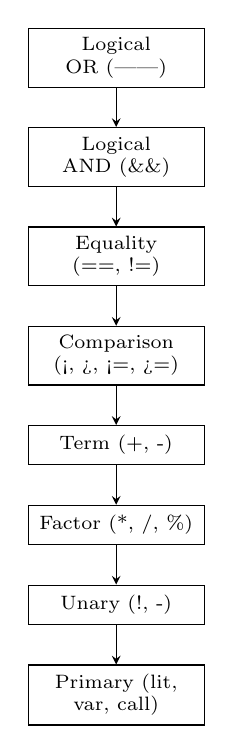
\begin{tikzpicture}[
    node distance=0.5cm,
    level/.style={rectangle, draw=black, text width=2cm, text centered, minimum height=0.5cm, font=\scriptsize},
    arrow/.style={->, >=stealth}
]
    \node[level] (or) {Logical OR (||)};
    \node[level, below=of or] (and) {Logical AND (\&\&)};
    \node[level, below=of and] (eq) {Equality (==, !=)};
    \node[level, below=of eq] (comp) {Comparison (<, >, <=, >=)};
    \node[level, below=of comp] (term) {Term (+, -)};
    \node[level, below=of term] (factor) {Factor (*, /, \%)};
    \node[level, below=of factor] (unary) {Unary (!, -)};
    \node[level, below=of unary] (primary) {Primary (lit, var, call)};
    
    \draw[arrow] (or) -- (and);
    \draw[arrow] (and) -- (eq);
    \draw[arrow] (eq) -- (comp);
    \draw[arrow] (comp) -- (term);
    \draw[arrow] (term) -- (factor);
    \draw[arrow] (factor) -- (unary);
    \draw[arrow] (unary) -- (primary);
\end{tikzpicture}
}
\caption{Recursive descent parser precedence hierarchy. Higher precedence operators are parsed first.}
\label{fig:precedence}
\end{figure}

\subsection{Semantic Analysis}

A symbol table is built using a hierarchical scope structure. Each scope uses a hash table for symbols, with parent pointers for proper scoping. The analyzer runs three passes: first, it adds functions and FFI declarations to the global scope; second, it analyzes each function body, adding variables and parameters to appropriate scopes during type checking; third, it detects unused variables and generates warnings.

Type checking verifies that operations use compatible types. Binary operations check operand compatibility, with automatic numeric promotions. Assignments verify type compatibility, allowing safe conversions but blocking unsafe ones.

Array bounds checking happens at two levels: compile-time for constant indices and runtime for dynamic indices. Bounds checking code is only generated when needed, eliminating checks for compile-time constant indices that are provably in bounds.

\begin{figure}[!t]
\centering
\scalebox{0.7}{
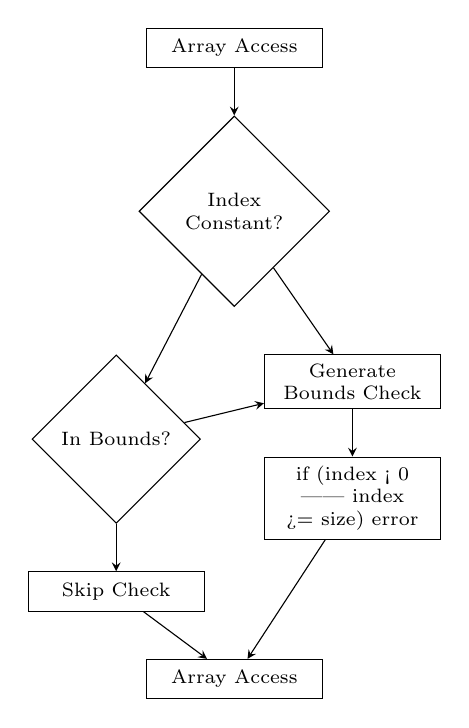
\begin{tikzpicture}[
    node distance=0.6cm,
    decision/.style={diamond, draw=black, text width=1.5cm, text centered, minimum height=0.6cm, font=\scriptsize},
    process/.style={rectangle, draw=black, text width=2cm, text centered, minimum height=0.5cm, font=\scriptsize},
    arrow/.style={->, >=stealth}
]
    \node[process] (start) {Array Access};
    \node[decision, below=of start] (const) {Index Constant?};
    \node[decision, below=of const, xshift=-1.5cm] (inbounds) {In Bounds?};
    \node[process, below=of inbounds] (skip) {Skip Check};
    \node[process, below=of const, xshift=1.5cm] (runtime) {Generate Bounds Check};
    \node[process, below=of runtime] (check) {if (index < 0 || index >= size) error};
    \node[process, below=of skip, xshift=1.5cm] (access) {Array Access};
    
    \draw[arrow] (start) -- (const);
    \draw[arrow] (const) -- (inbounds);
    \draw[arrow] (const) -- (runtime);
    \draw[arrow] (inbounds) -- (skip);
    \draw[arrow] (inbounds) -- (runtime);
    \draw[arrow] (runtime) -- (check);
    \draw[arrow] (check) -- (access);
    \draw[arrow] (skip) -- (access);
\end{tikzpicture}
}
\caption{Array bounds checking optimization. Compile-time constant indices are checked statically, eliminating runtime checks when safe.}
\label{fig:bounds_check}
\end{figure}

\begin{figure}[!t]
\centering
\scalebox{0.75}{
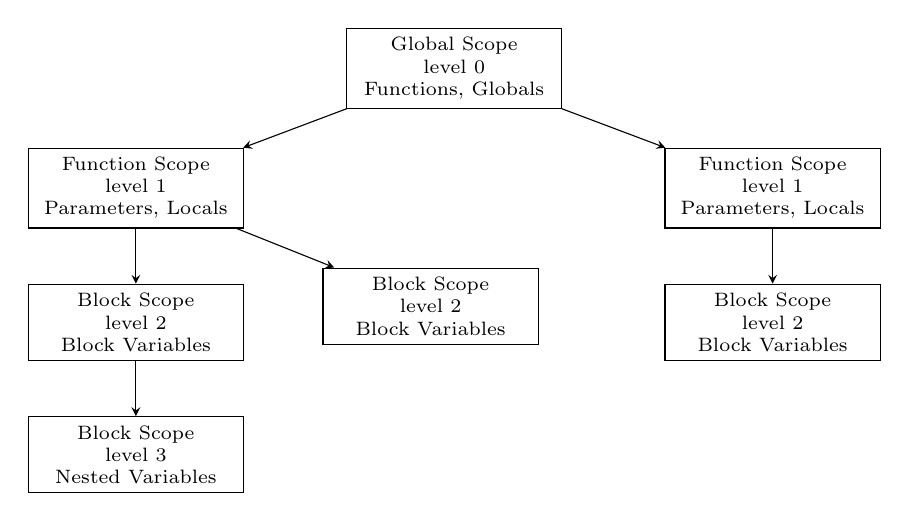
\begin{tikzpicture}[
    node distance=0.7cm,
    scope/.style={rectangle, draw=black, text width=2.5cm, text centered, minimum height=0.7cm, font=\scriptsize},
    arrow/.style={->, >=stealth}
]
    \node[scope] (global) {Global Scope\\level 0\\Functions, Globals};
    \node[scope, below left=of global, xshift=-0.8cm] (func1) {Function Scope\\level 1\\Parameters, Locals};
    \node[scope, below right=of global, xshift=0.8cm] (func2) {Function Scope\\level 1\\Parameters, Locals};
    \node[scope, below=of func1] (block1) {Block Scope\\level 2\\Block Variables};
    \node[scope, below right=of func1, xshift=0.5cm] (block2) {Block Scope\\level 2\\Block Variables};
    \node[scope, below=of func2] (block3) {Block Scope\\level 2\\Block Variables};
    \node[scope, below=of block1] (block4) {Block Scope\\level 3\\Nested Variables};
    
    \draw[arrow] (global) -- (func1);
    \draw[arrow] (global) -- (func2);
    \draw[arrow] (func1) -- (block1);
    \draw[arrow] (func1) -- (block2);
    \draw[arrow] (func2) -- (block3);
    \draw[arrow] (block1) -- (block4);
\end{tikzpicture}
}
\caption{Symbol table scope hierarchy. Each scope maintains a hash table of symbols and a pointer to its parent scope for symbol resolution.}
\label{fig:scopes}
\end{figure}

\subsection{IR Generation}

IR generation converts the annotated AST into three-address code. The IR has a simple instruction set covering arithmetic, comparisons, control flow, function calls, and memory operations.

Each function produces an \texttt{IRFunction} structure with the function name, return type, parameter list, instruction sequence, temporary variable counter, label counter for control flow, and loop context stack for break/continue handling.

Expression IR generation recursively processes AST nodes, generating instructions and temporaries as needed. Binary operations produce instructions with two operands and one result. Unary operations produce single-operand instructions. Function calls generate parameter passing instructions followed by call instructions.

Array indexing generates bounds checking code when the index isn't a compile-time constant or when the constant is out of bounds. Bounds checking uses conditional jumps to an error label generated once per function.

\begin{figure}[!t]
\centering
\scalebox{0.7}{
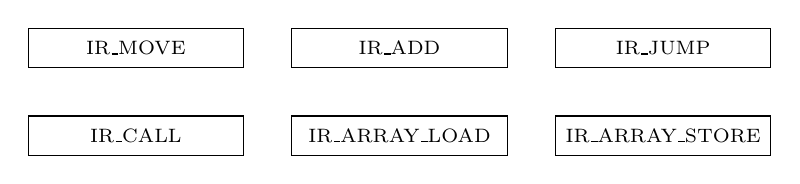
\begin{tikzpicture}[
    node distance=0.6cm,
    instr/.style={rectangle, draw=black, text width=2.5cm, text centered, minimum height=0.5cm, font=\scriptsize},
    arrow/.style={->, >=stealth}
]
    \node[instr] (move) {IR\_MOVE};
    \node[instr, right=of move] (add) {IR\_ADD};
    \node[instr, right=of add] (jump) {IR\_JUMP};
    \node[instr, below=of move] (call) {IR\_CALL};
    \node[instr, below=of add] (load) {IR\_ARRAY\_LOAD};
    \node[instr, below=of jump] (store) {IR\_ARRAY\_STORE};
\end{tikzpicture}
}
\caption{IR instruction format. Three-address code with at most two operands and one result per instruction.}
\label{fig:ir_instr}
\end{figure}

\begin{figure}[!t]
\centering
\scalebox{0.7}{
\begin{tikzpicture}[
    node distance=0.6cm,
    loop/.style={rectangle, draw=black, text width=2cm, text centered, minimum height=0.5cm, font=\scriptsize},
    stack/.style={rectangle, draw=black, dashed, text width=2cm, align=left, minimum height=0.4cm, font=\tiny},
    arrow/.style={->, >=stealth}
]
    \node[loop] (loop1) {Loop 1};
    \node[stack, below=0.1cm of loop1.south, anchor=north] (ctx1) {\hspace{0.05cm}start\_label\hspace{0.45cm}end\_label}
    \node[loop, below=of loop1] (loop2) {Loop 2};
    \node[stack, below=0.1cm of loop2.south, anchor=north] (ctx2) {\hspace{0.05cm}start\_label\hspace{0.45cm}end\_label}
    \node[loop, below=of loop2] (loop3) {Loop 3};
    \node[stack, below=0.2cm of loop3.south, anchor=north] (ctx3) {\hspace{0.05cm}start\_label\hspace{0.45cm}end\_label}
    
    \draw[arrow] (loop1) -- (loop2);
    \draw[arrow] (loop2) -- (loop3);
\end{tikzpicture}
}
\caption{Loop context stack for handling nested loops. Break and continue statements reference the current loop's labels.}
\label{fig:loop_stack}
\end{figure}

\subsection{Code Generation}

The Strategy design pattern is used for code generation, allowing switching between strategies for different target languages. The \texttt{CodeGenerator} structure holds IR program information and delegates target-specific work to strategy objects.

\subsubsection{C Code Generation}

The C code generator produces standard C code with appropriate type declarations and runtime support functions. Variable declarations use C types that match Twinkies types. Arrays get explicit sizes, and string operations use runtime library functions.

The C generator handles function declarations with proper C signatures, variable declarations with type conversions, control flow translation (if/while to C), array operations with bounds checking, string concatenation and manipulation, and FFI function declarations and dynamic loading.

Runtime functions include string manipulation (\texttt{\_\_tl\_concat}, \texttt{\_\_tl\_substr}, \texttt{\_\_tl\_strlen}, \texttt{\_\_tl\_strcmp}, \texttt{\_\_tl\_char\_at}), memory management, and error handling. These are generated automatically when needed and include null pointer checks and memory allocation.

\subsubsection{Assembly Code Generation}

The assembly generator produces x86-64 assembly code. It handles register allocation, calling conventions, and platform-specific syntax. The assembly generator works but is more experimental than the C generator.

\subsubsection{FFI Code Generation}

FFI code generation produces platform-specific code for dynamic library loading. On Windows, \texttt{LoadLibrary} and \texttt{GetProcAddress} are used. On Linux and macOS, \texttt{dlopen} and \texttt{dlsym} are used. Function pointers are generated with appropriate calling conventions (cdecl, stdcall, etc.).

The FFI system supports multiple calling conventions for compatibility with different libraries. Supported conventions include \texttt{cdecl} (default C), \texttt{stdcall} (Windows API), \texttt{fastcall} (optimized), and \texttt{thiscall} (C++ member functions). The compiler generates function pointer type definitions with the right calling convention prefixes (\texttt{\_\_cdecl}, \texttt{\_\_stdcall}, \texttt{\_\_fastcall}) based on the source declaration.

The FFI system supports multiple library types: \texttt{DLL} for Windows, \texttt{SO} for Linux, \texttt{DYLIB} for macOS, and \texttt{STATIC} for static libraries. The compiler resolves library paths based on the platform, adding the right extensions (\texttt{.dll}, \texttt{.so}, \texttt{.dylib}, or \texttt{.a}).

Platform-specific implementations differ:
\begin{itemize}
    \item \textbf{Windows}: Uses \texttt{LoadLibraryA} for loading and \texttt{GetProcAddress} for symbol resolution. Unloads with \texttt{FreeLibrary}.
    \item \textbf{Linux}: Uses \texttt{dlopen} with \texttt{RTLD\_LAZY} for lazy binding, \texttt{dlsym} for symbol resolution, and \texttt{dlclose} for unloading.
    \item \textbf{macOS}: Similar to Linux, uses \texttt{dlopen}, \texttt{dlsym}, and \texttt{dlclose} with platform-specific path resolution for \texttt{.dylib} files.
\end{itemize}

The generated C code includes a \texttt{load\_ffi\_functions()} function called at program startup. It loads each required library once, resolves all function symbols, and stores them in function pointer variables prefixed with \texttt{ffi\_}. Error handling is generated for cases where libraries fail to load or symbols can't be resolved, with error messages and program termination.

\subsubsection{Inline Assembly}

Twinkies supports inline assembly statements that allow embedding platform-specific assembly code directly in source programs. The syntax follows GCC-style inline assembly with support for output operands, input operands, and clobber lists.

Inline assembly statements use the \texttt{asm} keyword followed by an optional \texttt{volatile} modifier and a block containing assembly code strings. The syntax is: \texttt{asm \{ "assembly code" : outputs : inputs : clobbers \}}. The \texttt{volatile} modifier prevents the compiler from optimizing away the assembly code, which is useful for memory barriers, CPUID instructions, and other side-effect operations.

Output operands specify variables that receive values from the assembly code. Each output uses the format \texttt{"constraint" (variable)}, where constraints like \texttt{"=r"} (register output) or \texttt{"=a"} (EAX/RAX register) control register allocation. Input operands pass values from Twinkies variables into the assembly code using similar constraint syntax. Clobber lists declare registers or memory that the assembly code modifies, preventing the compiler from using those resources for other operations.

The parser recognizes inline assembly statements and extracts the assembly code string, volatile flag, and operand lists. Semantic analysis passes inline assembly through without type checking, since the assembly code is trusted. IR generation creates \texttt{IR\_INLINE\_ASM} instructions that preserve the assembly code and operand information. C code generation translates these into GCC-style \texttt{\_\_asm\_\_} or \texttt{\_\_asm\_\_ \_\_volatile\_\_} statements with proper operand constraints and clobber lists.

Inline assembly enables low-level operations like CPUID for processor information, RDTSC for timing, bit manipulation instructions, and direct memory access. The generated C code uses the same inline assembly syntax, allowing the C compiler to handle register allocation and optimization while preserving the assembly semantics.

\begin{figure}[!t]
\centering
\scalebox{0.75}{
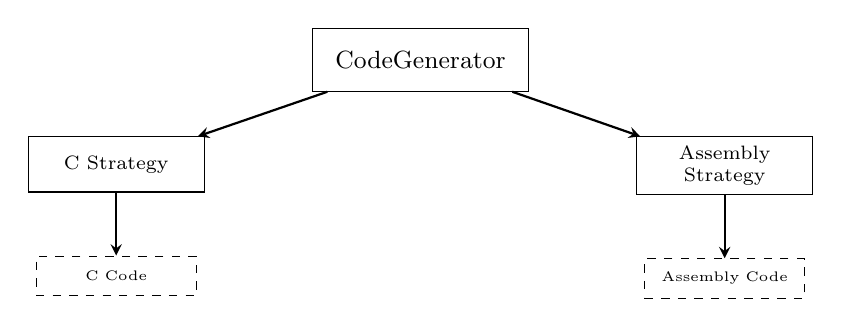
\begin{tikzpicture}[
    node distance=0.8cm,
    strategy/.style={rectangle, draw=black, text width=2cm, text centered, minimum height=0.7cm, font=\scriptsize},
    generator/.style={rectangle, draw=black, text width=2.5cm, text centered, minimum height=0.8cm, font=\small},
    output/.style={rectangle, draw=black, dashed, text width=1.8cm, text centered, minimum height=0.5cm, font=\tiny},
    arrow/.style={->, >=stealth, thick}
]
    \node[generator] (codegen) {CodeGenerator};
    \node[strategy, below left=of codegen, xshift=-0.8cm] (cstrat) {C Strategy};
    \node[strategy, below right=of codegen, xshift=0.8cm] (asmstrat) {Assembly Strategy};
    
    \node[output, below=of cstrat] (cout) {C Code};
    \node[output, below=of asmstrat] (asmout) {Assembly Code};
    
    \draw[arrow] (codegen) -- (cstrat);
    \draw[arrow] (codegen) -- (asmstrat);
    \draw[arrow] (cstrat) -- (cout);
    \draw[arrow] (asmstrat) -- (asmout);
\end{tikzpicture}
}
\caption{Strategy pattern in code generation. The CodeGenerator delegates target-specific operations to strategy objects.}
\label{fig:strategy}
\end{figure}

\section{Evaluation}

The Twinkies compiler was evaluated through correctness testing and performance analysis. The test suite includes examples covering basic language features, advanced constructs, FFI integration, and error cases.

\subsection{Test Suite Organization}

Test suites are organized by category: basic tests for arithmetic, control flow, and I/O; advanced tests for arrays, functions, and type conversions; FFI tests for foreign function integration; module tests for the module system and headers; and debugging tests for error cases and edge conditions.

\subsection{Correctness Testing}

All test cases compile successfully and produce expected output. The compiler handles type checking with proper error messages, array bounds checking at compile-time and runtime, scope resolution and variable shadowing, function overloading and parameter matching, FFI calls with proper calling conventions, and module imports and symbol resolution.

\subsection{Error Detection}

The compiler detects and reports various error types: syntax errors with location information, type mismatches with suggestions, undefined variable references, array bounds violations, and invalid operations on incompatible types.

Error messages include line and column numbers, error context, and suggestions when applicable. This gives a better developer experience than cryptic compiler errors.

\subsection{Performance Considerations}

As a transpiler, performance is measured by compilation speed, not generated code performance. The compiler processes typical programs (under 1000 lines) in milliseconds, which works well for interactive development.

Generated C code benefits from standard C compiler optimizations when compiled with optimization flags. The IR could be extended with optimization passes, but the current implementation prioritizes correctness over optimization.

\section{Discussion}

\subsection{Design Trade-offs}

Several design decisions trade simplicity for features:

\textbf{Hand-written vs. Generated Parsers}: The recursive descent parser gives better error messages and is easier to debug than generated parsers, but it needs more maintenance as the language evolves.

\textbf{Three-Address IR}: The simple IR format is easy to generate and translate, but it lacks the expressiveness needed for advanced optimizations. Future work could add a more sophisticated IR with SSA form.

\textbf{Strategy Pattern}: The strategy pattern adds some indirection overhead, but it provides clear separation of concerns and makes adding new target languages straightforward.

\subsection{Limitations}

The current implementation has several limitations: (i) no optimization passes in the IR, (ii) limited error recovery in the parser, (iii) assembly generation is experimental, (iv) no garbage collection for string types, and (v) the module system doesn't detect circular dependencies.

\subsection{Lessons Learned}

Compiler construction needs careful attention to error handling and reporting. Investing in comprehensive error messages pays off during development and debugging. The modular architecture allows adding features incrementally without major refactoring.

The Strategy pattern worked well for multi-target code generation, allowing independent development of different code generators. This separation also makes testing easier, since each strategy can be tested on its own.

\section{Conclusion and Future Work}

This paper presented the design and implementation of the Twinkies compiler, a complete compilation system with static type checking, FFI integration, and multi-target code generation. The compiler shows that a clean, modular architecture leads to maintainable compiler construction and robust error detection.

The compiler handles a wide range of language features, from basic arithmetic to complex FFI integration. The test suite validates correctness across diverse use cases, and the error reporting system provides helpful diagnostics.

Future work includes: (i) IR optimization passes like constant folding and dead code elimination, (ii) SSA form for more advanced optimizations, (iii) improved error recovery in the parser, (iv) garbage collection for automatic memory management, (v) additional target languages including LLVM IR and WebAssembly, (vi) incremental compilation for large projects, and (vii) language server protocol support for IDE integration.

The Twinkies compiler works as both a practical tool and a demonstration of modern compiler techniques. The codebase provides a foundation for further research in language design and compilation strategies.

\begin{thebibliography}{00}
\bibitem{aho2006compilers} A. V. Aho, M. S. Lam, R. Sethi, and J. D. Ullman, \textit{Compilers: Principles, Techniques, and Tools}, 2nd ed. Boston, MA, USA: Pearson Education, 2006.

\bibitem{lesk1975lex} M. E. Lesk and E. Schmidt, ``Lex—A Lexical Analyzer Generator,'' Bell Laboratories, Murray Hill, NJ, USA, Tech. Rep., 1975.

\bibitem{grune2012parsing} D. Grune and C. J. H. Jacobs, \textit{Parsing Techniques: A Practical Guide}, 2nd ed. New York, NY, USA: Springer, 2012.

\bibitem{cooper2011engineering} K. D. Cooper and L. Torczon, \textit{Engineering a Compiler}, 2nd ed. San Francisco, CA, USA: Morgan Kaufmann, 2011.

\bibitem{meyer1997object} B. Meyer, \textit{Object-Oriented Software Construction}, 2nd ed. Upper Saddle River, NJ, USA: Prentice Hall, 1997.

\bibitem{gamma1994design} E. Gamma, R. Helm, R. Johnson, and J. Vlissides, \textit{Design Patterns: Elements of Reusable Object-Oriented Software}. Boston, MA, USA: Addison-Wesley, 1994.

\bibitem{levy2017ownership} A. Levy, ``Ownership and Borrowing in Rust,'' in \textit{Proc. ACM SIGPLAN Int. Conf. Object-Oriented Programming, Systems, Languages, and Applications}, 2017, pp. 1--15.
\end{thebibliography}

\end{document}